\section{Results}
\label{sec:result}

In this section we discuss the implementation and performance comparison of the different NoC implementations.
All designs are modeled using Verilog HDL and extensively simulated for their functional correctness.
We use the CONNECT open-source NoC platform as the fat tree and mesh references~\cite{papa_connect_fpga2012}.
The designs are simulated as well as implemented with Vivado 2017.3 targeting Xilinx xc7vx690t FPGA (VC709 evaluation board).

\input Tables/SystemResource
Table~\ref{table:systemResourceConsumption} compares the resource utilization and the maximum frequency of operation for the binary tree, AsyncBTree, and fat tree for different network sizes.
As expected binary trees are least resource intensive due to their simple switch architecture.
AsyncBTree consumes 45\% to 65\% more LUTs and about 165\% more flip flops compared to the binary tree implementation.
The multiple frequencies in the HNoC column represent the maximum clock frequency supported at different tree levels.
At the lowest level (switches connected to PEs), the clock performance is better than that of binary trees but deteriorates as going higher in the hierarchy.
This could be because of the additional pipelining present inside the asynchronous FIFOs.
This also means if AsyncBTree is used as a synchronous NoC (all tree levels are clocked by a single clock source), its resource consumption and performance will be worse than a binary tree. 

Compared to AsyncBTree, fat trees consumes $\sim$3.7$\times$ LUTs but less than half the number of flip flops.
AsyncBTree requires more flip flops due to the presence of asynchronous FIFOs.
For fat trees, the impact due to complex switches can be clearly seen in the clock performance, where they are not even able to achieve 200 MHz for a high-end FPGA.
Due to the low clock performance of the NoC, the PEs also have to be under-clocked in most scenarios for overall synchronous operations.
%Otherwise synchronization FIFOs have to be inserted between PEs and the NoC switches, which will further increase the resource utilization.
Considering the fact that the number of LUTs available in 7-series Xilinx FPGAs are half of that of number of flip-flops, HNoC is much lite compared fat trees at the same time given more than 4$\times$ clock performance.


\begin{figure*}[t]
\centering     %%% not \center
\subfigure[Random]{\label{fig:randtput}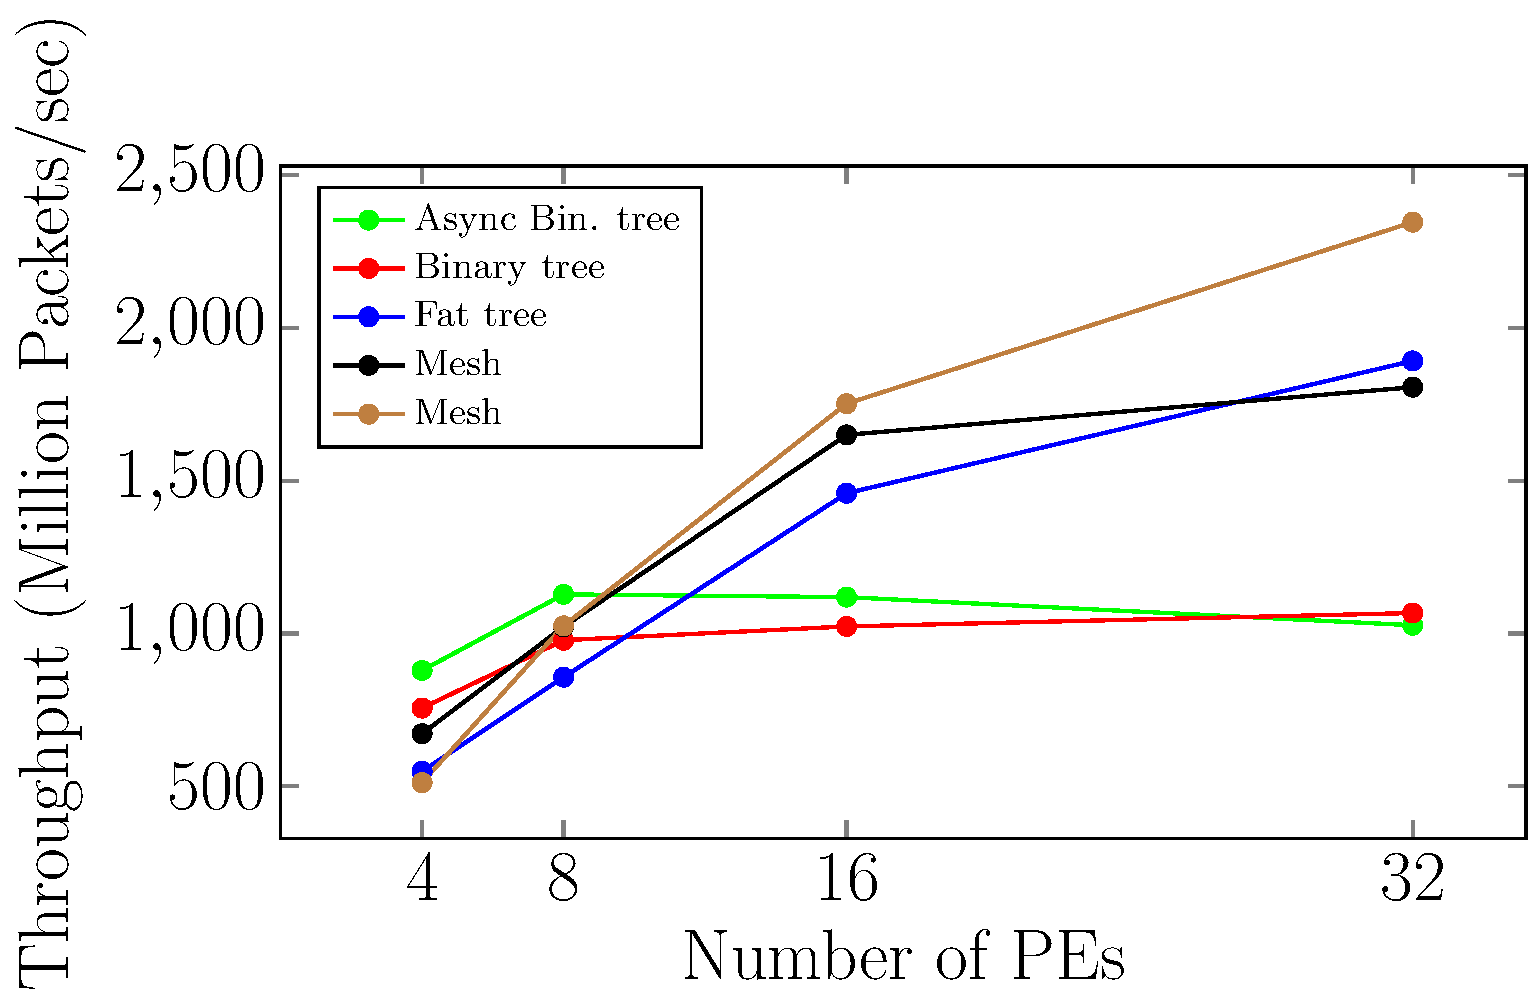
\includegraphics[width=0.55\columnwidth]{Data/randomTputMax.pdf}}
\subfigure[Tornado]{\label{fig:torndadotput}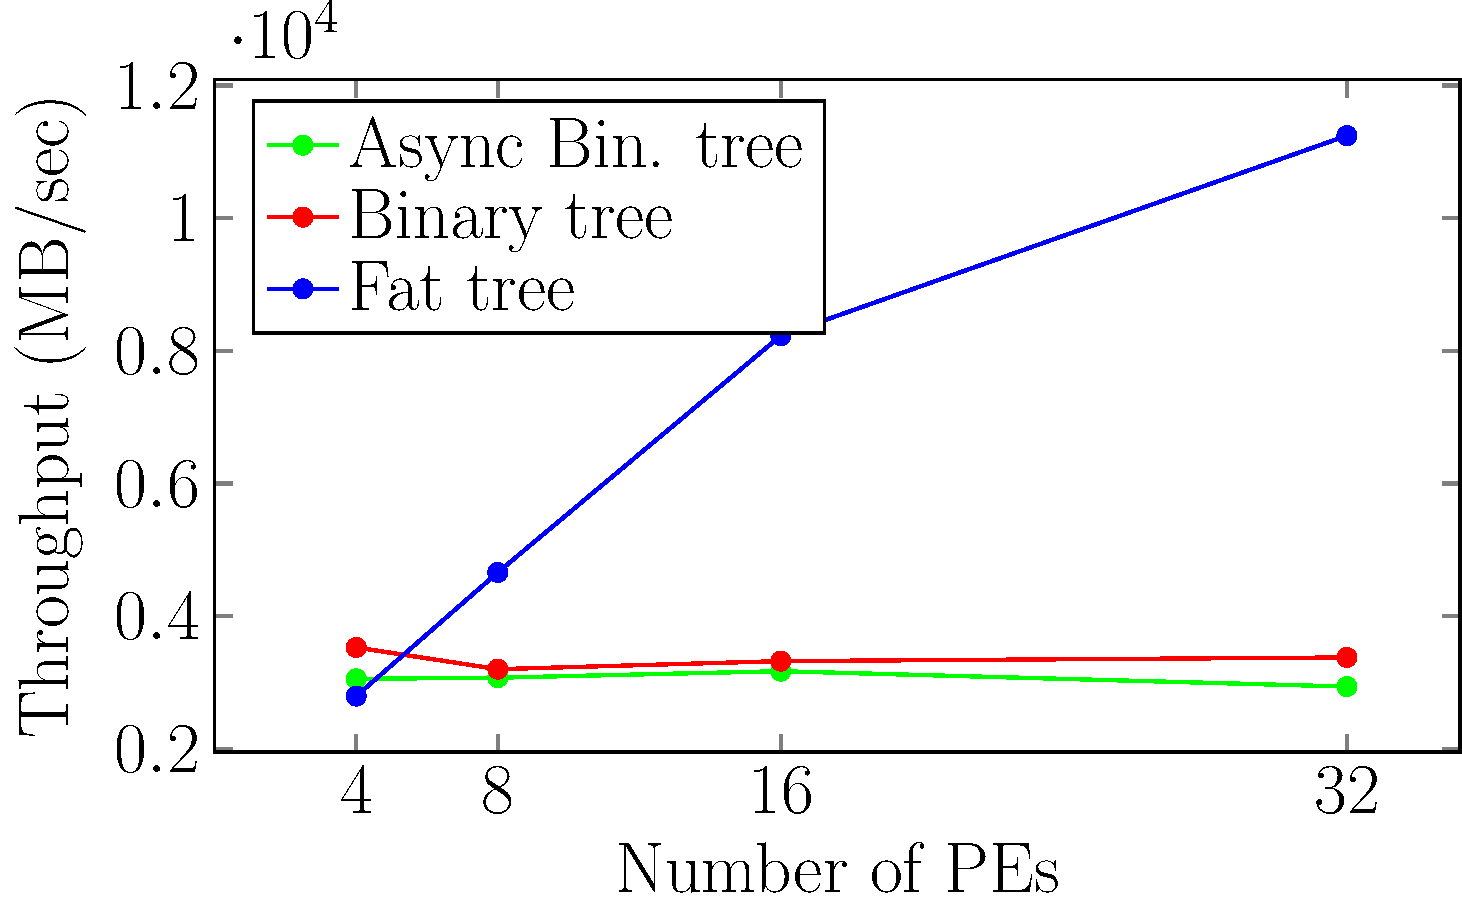
\includegraphics[width=0.55\columnwidth]{Data/tornadoTputMax.pdf}}
%\subfigure[Complement]{\label{fig:complementtput}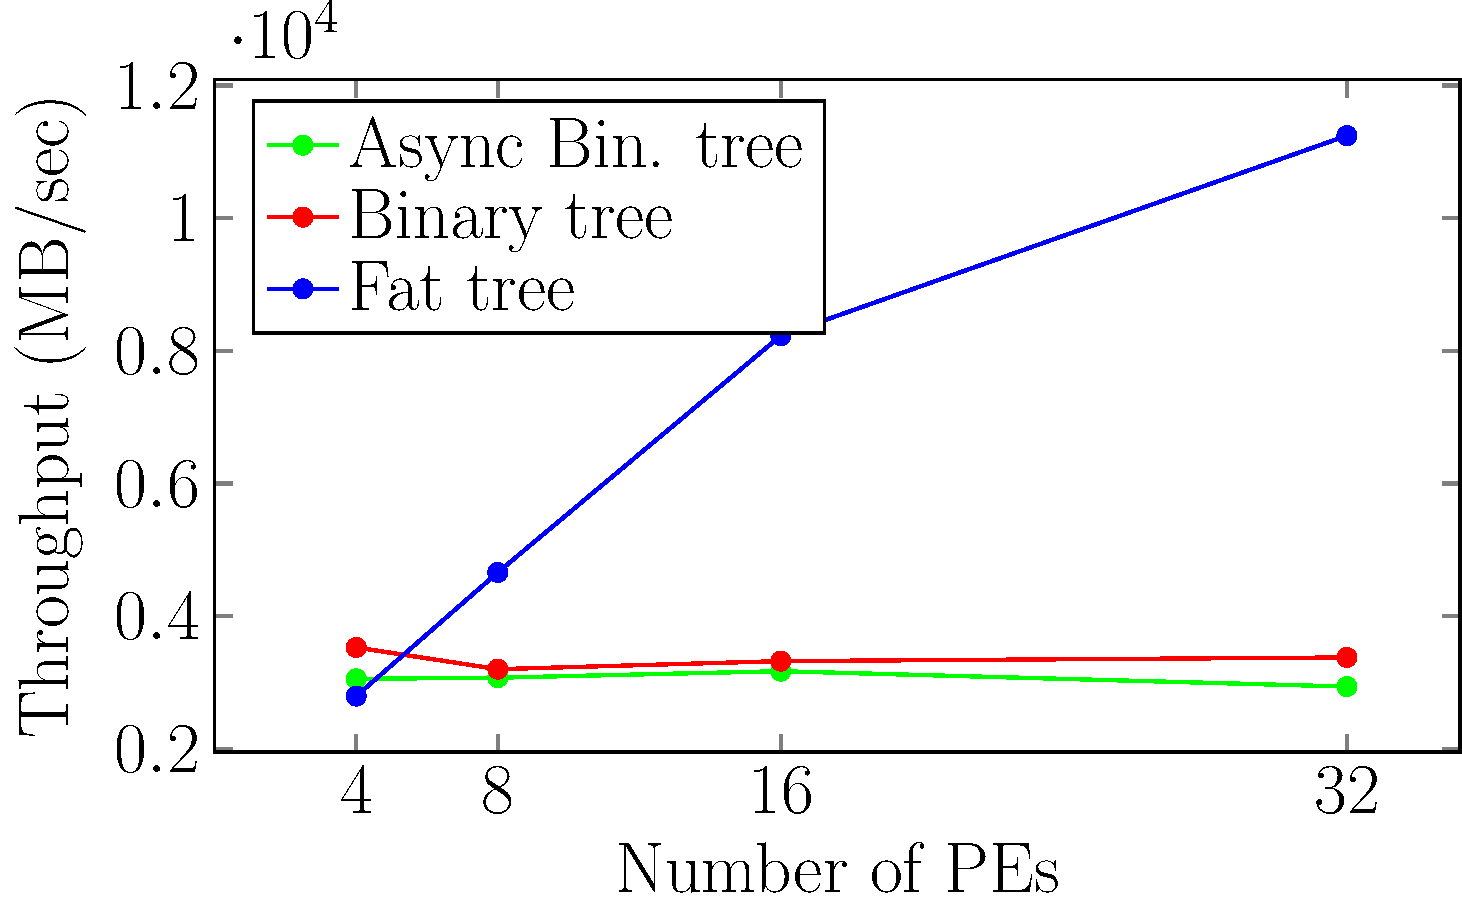
\includegraphics[width=0.5\columnwidth]{Data/complementTputMax.pdf}}
\subfigure[Reverse]{\label{fig:reversetput}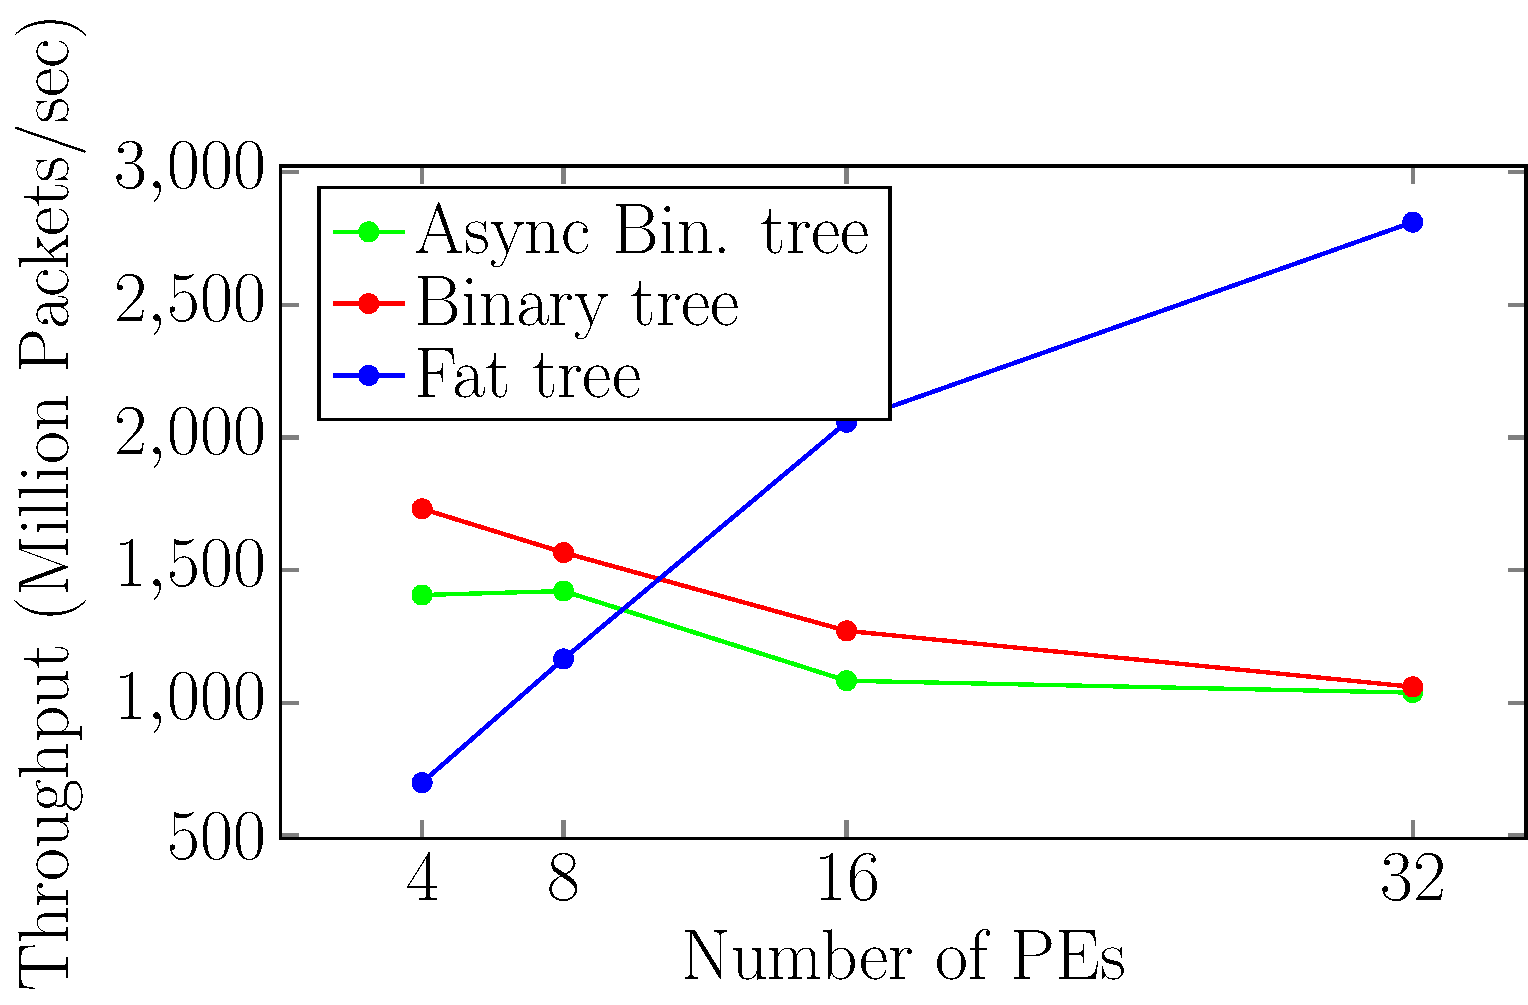
\includegraphics[width=0.55\columnwidth]{Data/reverseTputMax.pdf}}
\vspace{-3mm}
\caption{Throughput of different Binary NoC architectures with varying size corresponding to different traffic patterns}
\vspace{-5mm}
\label{fig:tputmax}
\end{figure*}

\begin{figure*}[t]
\centering     %%% not \center
\subfigure[Random]{\label{fig:rndlatency}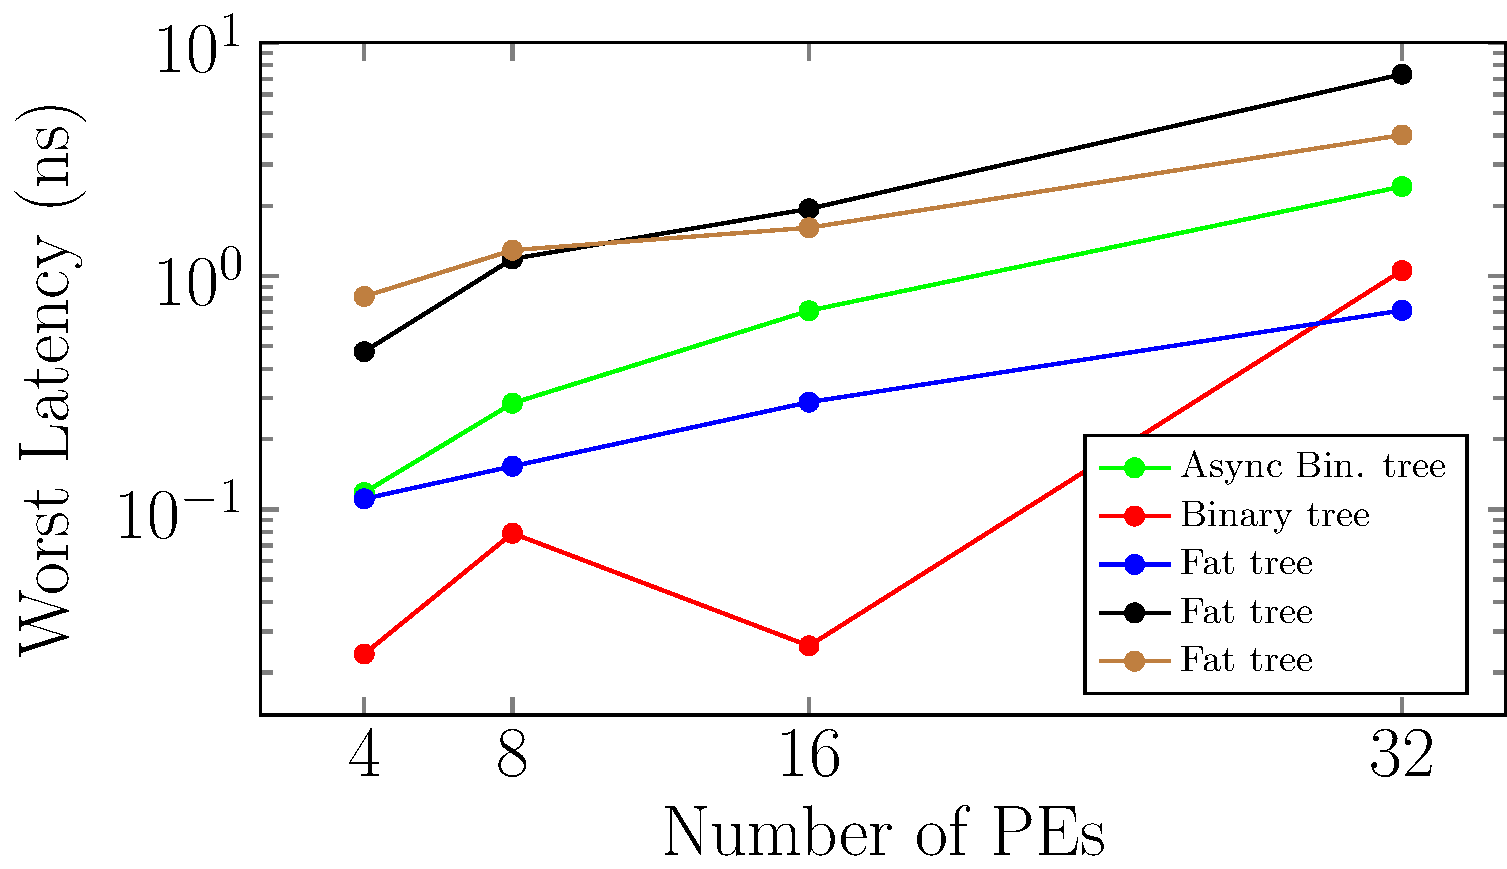
\includegraphics[width=0.55\columnwidth]{Data/randomLatencyMax.pdf}}
\subfigure[Tornado]{\label{fig:tornadolatency}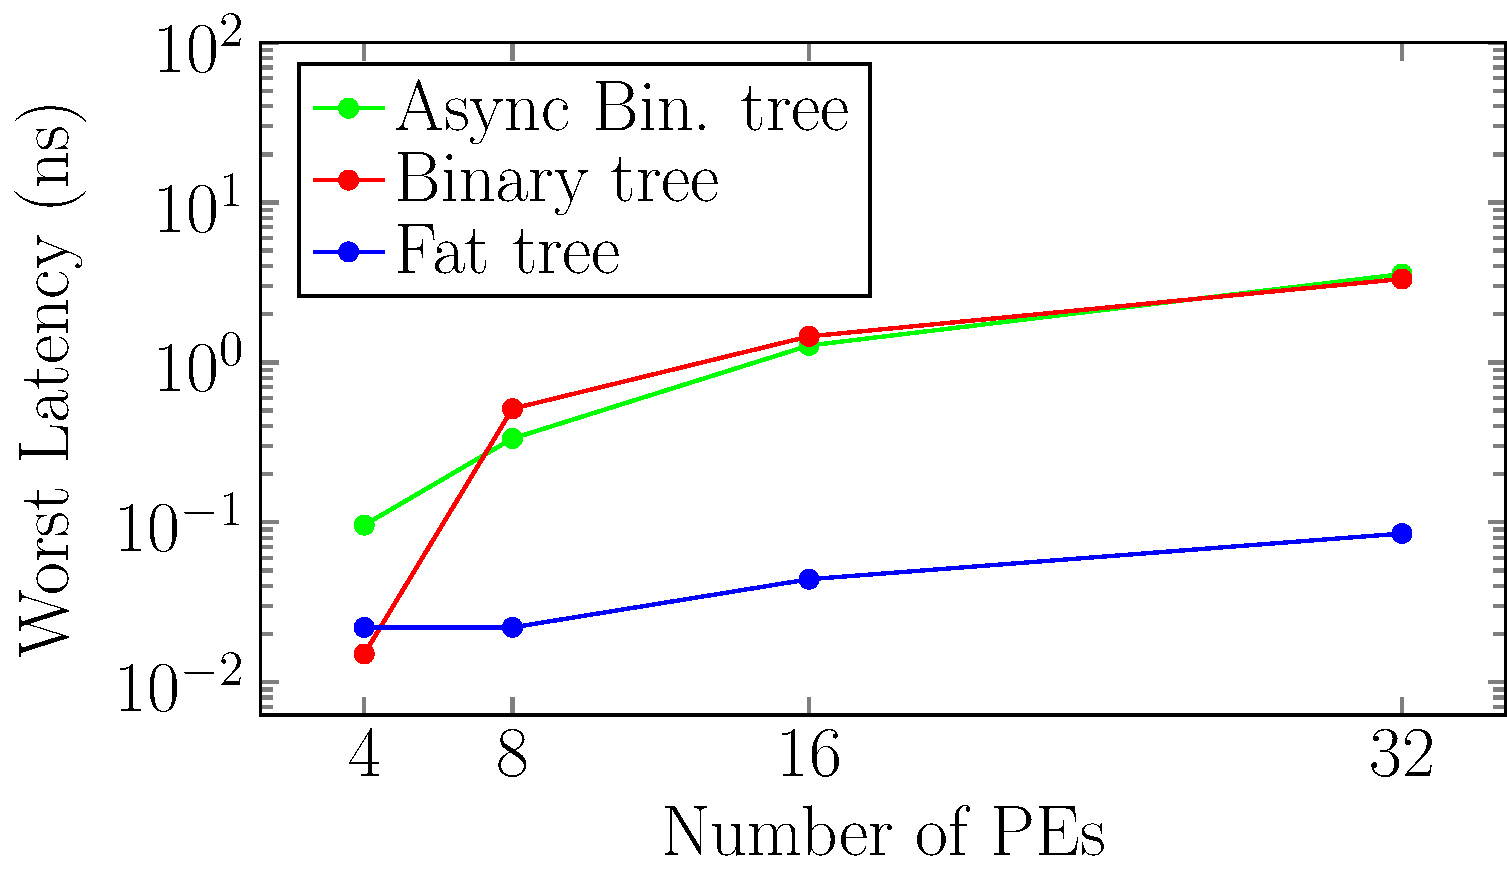
\includegraphics[width=0.55\columnwidth]{Data/tornadoLatencyMax.pdf}}
%\subfigure[Complement]{\label{fig:complementlatency}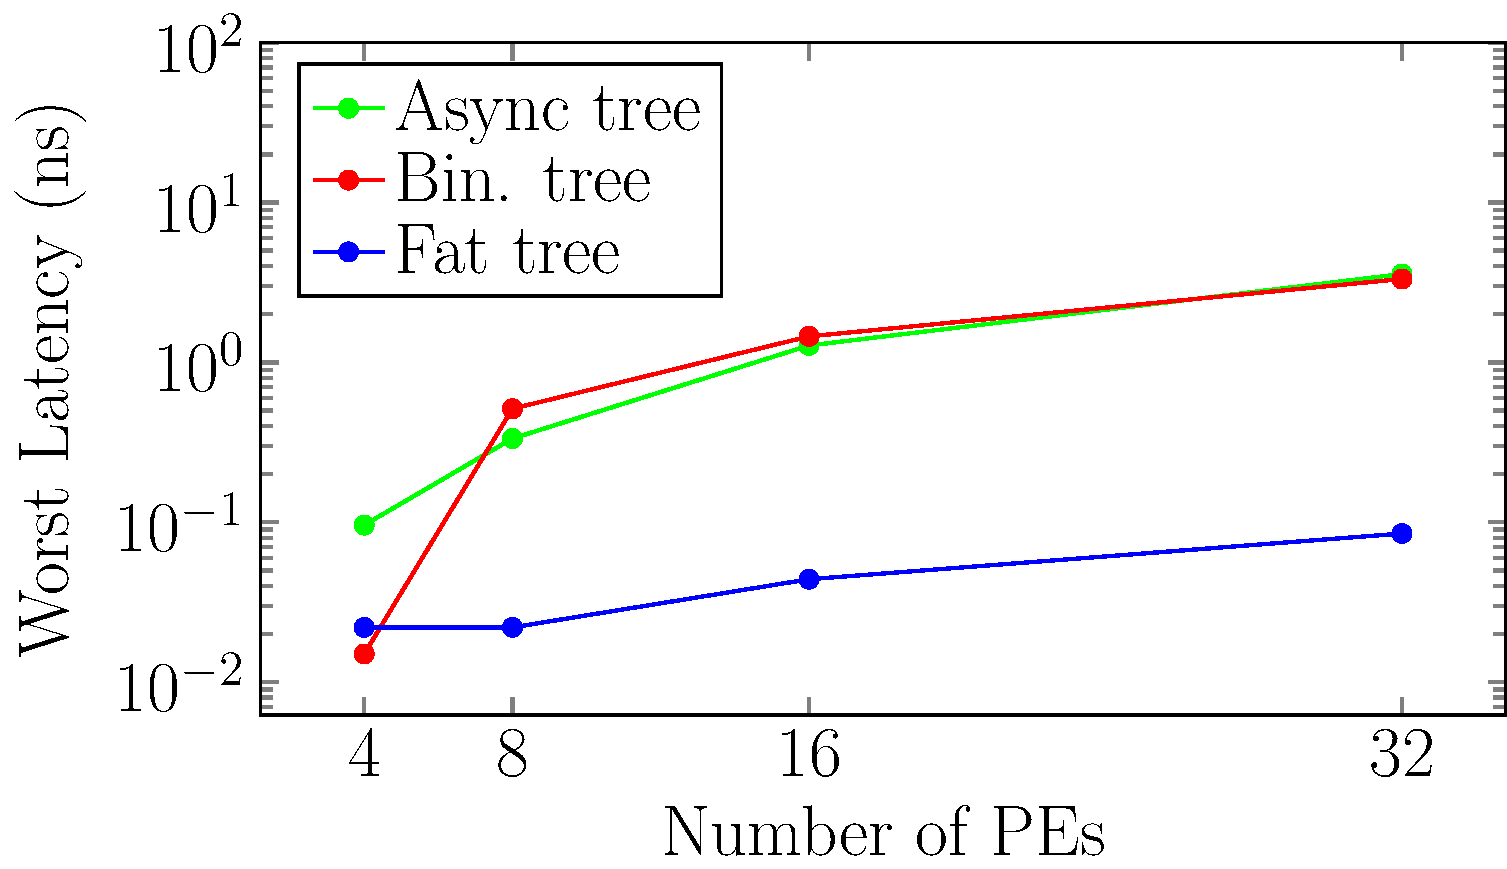
\includegraphics[width=0.5\columnwidth]{Data/complementLatencyMax.pdf}}
\subfigure[Reverse]{\label{fig:reverselatency}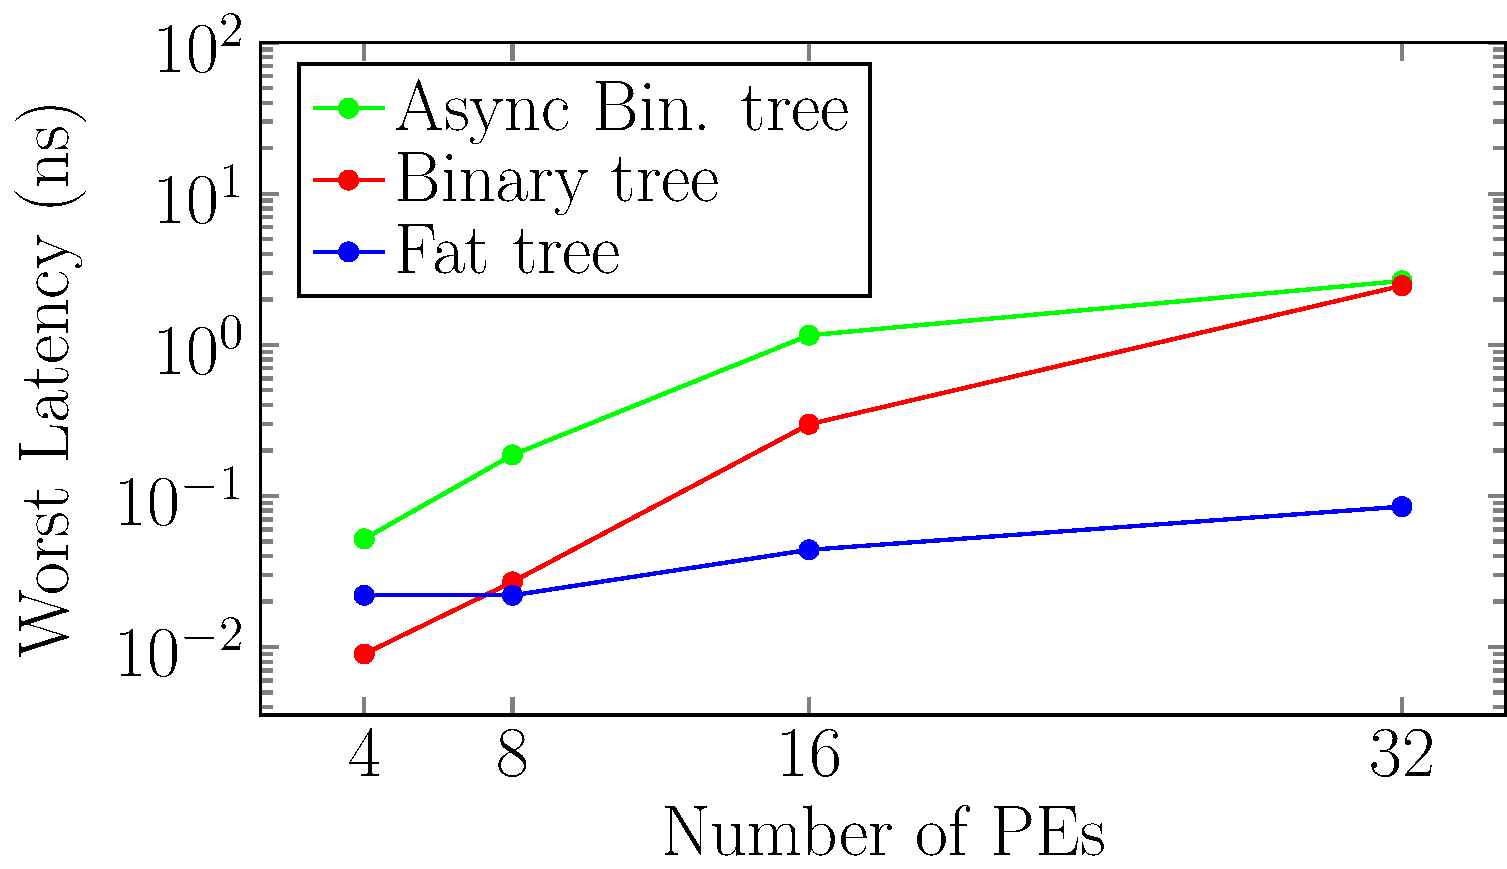
\includegraphics[width=0.55\columnwidth]{Data/reverseLatencyMax.pdf}}
\vspace{-3mm}
\caption{Maximum latency of different Binary NoC architectures with varying size corresponding to different traffic patterns}
\vspace{-5mm}
\label{fig:latmax}
\end{figure*}

Fig.~\ref{fig:tput} and~\ref{fig:latency} compares the throughput and latency of the three implementations with different NoC sizes for different traffic patterns such as random, tornado and reverse.
In each case, the PE to switch interface is clocked at the lowest frequency supported by the three implementations.
For HNoC upper levels are clocked at double the frequency of lower levels, but limited by maximum supported frequency shown in Table~\ref{table:systemResourceConsumption}.
It could be seen that for NoC size up to 8 PEs, HNoC performance is better than or comparable to that of fat trees.
For larger tree sizes, fat trees perform better since the clock frequencies cannot be scaled beyond a limit.
If PEs run at lower clock frequencies ($\sim$50 MHz), AsyncBTree can provide better performance for NoC with up to 16 PEs. 

Fig.~\ref{fig:tputmax} and~\ref{fig:latmax} compares the throughput and latency when each implementation is running at its maximum supported frequency.
Again for smaller NoC sizes binary tree and AsyncBTree out performs fat tree for random traffic pattern.
But for larger NoC sizes fat trees are clearly advantageous.
Fig.~\ref{fig:tputmax}(a) also shows the performance of mesh topology, which is the most popular NoC topology, compared to different tree topologies.
Again for smaller NoC sizes (8 or less) AsyncTree performance is better.
Several FPGA-based multi-processor systems have 8 core or less thus AsyncBTree could be much suitable for their implementation.

Fig.~\ref{fig:tputPerf} compares the performance of each NoC compared to their resource utilization.
Synchronous binary trees clearly have an upper hand in this regard.
AsyncBtree give moderately high throughput by consuming relatively less resources.
But for larger NoC size, mesh topology is still the suitable candidate.


\begin{figure}[t]
\centering
   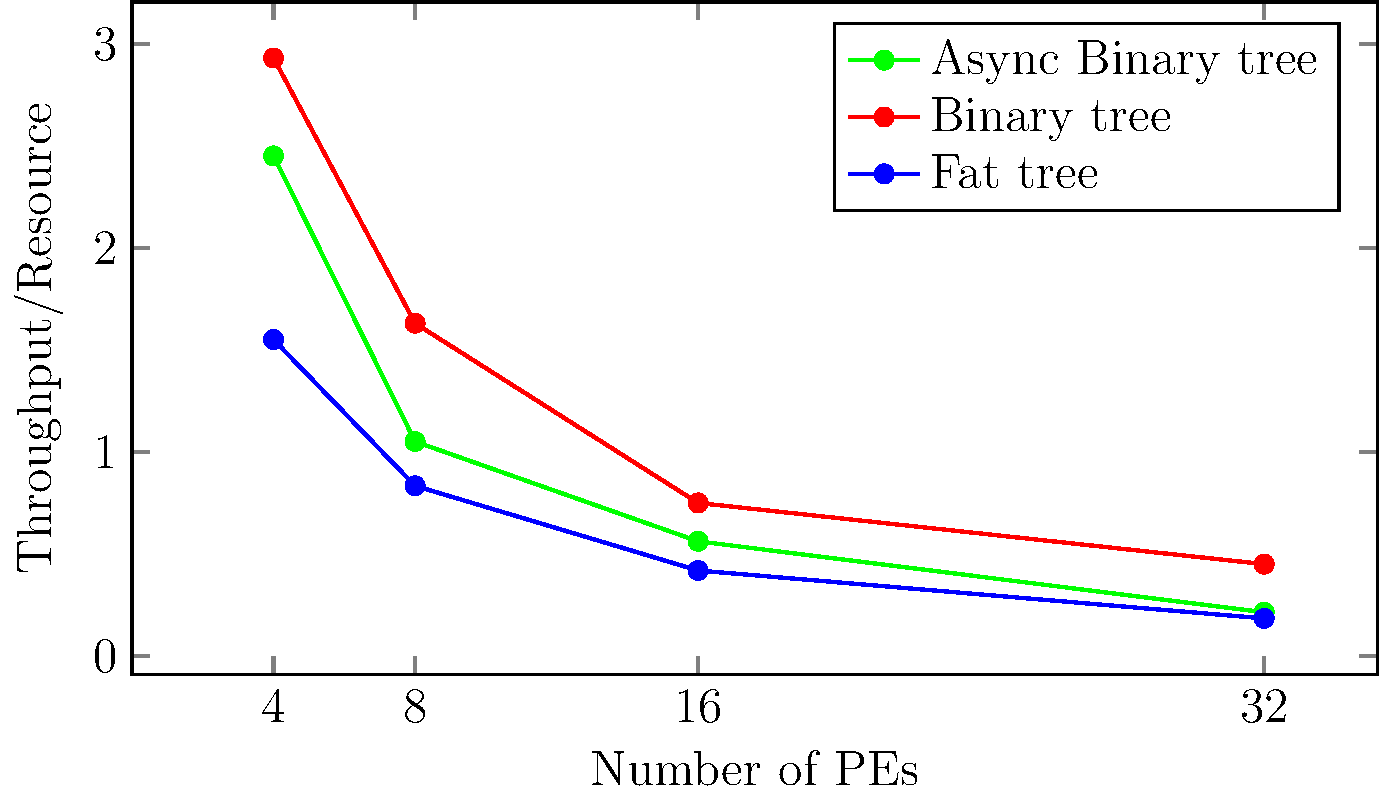
\includegraphics[width=0.6\columnwidth]{Data/tputVsCost.pdf}
         \vspace{-2mm}
   \caption{Throughput vs cost}
      \vspace{-5mm}
      \label{fig:tputPerf}
\end{figure}
